\documentclass[aspectratio=169, 12pt]{beamer}

\usetheme[progressbar=frametitle]{metropolis}
\usepackage{appendixnumberbeamer}

\usepackage{booktabs}
\usepackage{svg}
\usepackage[scale=2]{ccicons}

\usepackage{pgfplots}
\usepgfplotslibrary{dateplot}

\usepackage{xspace}
\newcommand{\themename}{\textbf{\textsc{metropolis}}\xspace}

\title{Forex Forecasting}
\subtitle{Combining statistical methods with neural networks}
% Authors
\author{Eustathios Kotsis \inst{1} \and Darmanis Michael \inst{1} \and Vasilios Venieris \inst{1}}
% Affiliations
\institute{\inst{1} National and Kapodistrian University of Athens}
% Date
\date{\today}
% \institute{Center for modern beamer themes}
% \titlegraphic{\hfill\includegraphics[height=1.5cm]{logo.pdf}}

\begin{document}

\maketitle

\section{Smoothed Convolutional Neural Network (S-CNN)}

\begin{frame}{S-CNN: Origin and basic idea}
    \begin{itemize}
        \item Implementation based on the paper ``Time-series analysis with smoothed Convolutional Neural Network''\cite{e-cnn} .
        \item Model is univariate, multi-step.
        \item Simple exponential smoothing (remove outliers, average) + CNN.
    \end{itemize}
\end{frame}

\begin{frame}[allowframebreaks]{S-CNN: Simple Exponential Smoothing}
  \begin{equation*}
    \displaystyle s_{t}=\alpha x_{t}+(1-\alpha )s_{t-1}=s_{t-1}+\alpha (x_{t}-s_{t-1})
  \end{equation*}
    \begin{itemize}
        \item For $\alpha$ values close to 1 we get very little influence of the previous smoothed value.
        \item For $\alpha$ close to 1 we also see that the previous unsmoothed series observation influences the result more than the smoothed values.
        \item For the calculation of $\alpha$, since there is no golden rule, we adopted the $\alpha$ value from the aforementioned publication.
        \item In particular the authors argue that $\alpha$ should be dependent on the dataset and must be of course between 0 and 1. Also the average value of the series should be less than the difference between max and min.
    \end{itemize}
So we end up with the following formula
\begin{equation*}
\alpha_{\text{Optimum}} = \frac{\left( X_{\text{max}} - X_{\text{min}} \right) - \frac{1}{n} \sum_{t=1}^{n} X_t}{X_{\text{max}} - X_{\text{min}}},
\end{equation*}
and the simple smoothing becomes
\begin{equation*}
S_t = S_{t-1} + \frac{\left( X_{\text{max}} - X_{\text{min}} \right) - \frac{1}{n} \sum_{t=1}^{n} X_t}{X_{\text{max}} - X_{\text{min}}} \left( X_t - S_{t-1} \right) .
\end{equation*}
\end{frame}

\begin{frame}{S-CNN: Architecture}
Basic architecture from Wibawa et al.\cite{e-cnn} and experimented with different number of hidden layers.
\begin{figure}[htbp]
\centering
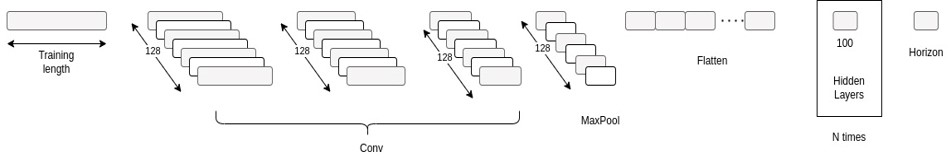
\includegraphics[width=\columnwidth]{./plots/s-cnn.jpg}
\end{figure}
\end{frame}

\begin{frame}[allowframebreaks]{S-CNN: Training}
    \begin{center}
    \textsc{\textbf{How to pick the number of hidden layers?}}
    \end{center}
    We used the Lucas numbers suggested.They derive from the Fibonacci Sequence if instead of adding every 2 successive observations we skip the intermediate and add the K with the K+2 together.
    \begin{figure}[htbp]
    \centering
    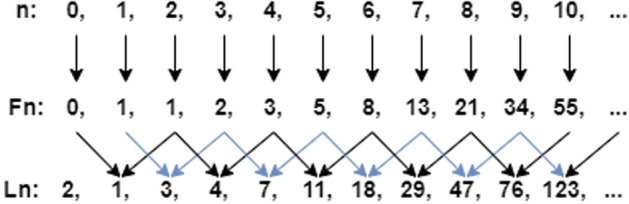
\includegraphics[width=0.6\columnwidth]{./plots/fibonacci.jpg}
    \end{figure}

Model yielded the lower MSE, for the most stable currencies, for 76 layers of training.

\begin{table}[htbp]
\centering
\caption{Training time for different numbers of hidden layers}
\begin{tabular}{cc}
\toprule
Number of Hidden Layers & Training Time (hh:mm:ss) \\
\midrule
3 & 0:27:43.15 \\
11 & 0:34:27.77 \\
47 & 1:05:21.78 \\
76 & 1:28:47.70 \\
\bottomrule
\end{tabular}
\end{table}
\begin{center}
    \textsc{\textbf{Training steps...}}
\end{center}
\begin{itemize}
\item Split the dataset into series of different frequencies.
\item For each time series we normalise + smooth.
\item Feed the output into the convolutional model and train the model to predict a horizon of K steps for this frequency, where K is a model’s designers choice.
\end{itemize}
\newpage
\begin{center}
    \textsc{\textbf{Training history.}}
\end{center}
In order to balance training with only recent data, or feeding with irrelevant outdated history, we train with a list of possible training lengths.
\begin{itemize}
    \item Daily: [14, 20, 240]
    \item Weekly: [52, 13, 26]
    \item Monthly: [24, 18]
    \item Quarterly: [12, 8]
    \item Yearly: [6]
\end{itemize}
\newpage
\begin{center}
    \textsc{\textbf{Train/validation/test split.}}
\end{center}
\begin{itemize}
    \item We focused on data after 2010 since in 2008 – 2010 there was the European debt crisis. A plot from the data can show that the economy and the currency fell rapidly in most countries in the European continent and in many other countries.
    \item For the frequencies except Yearly, we trained with splits of 80\%-20\%, 70\%-30\%, and approximately 60\%-40\% for quarterly (training/validation).
    \item We split the dataset accordingly and fed the created datasets to the generators.
    \item The models were trained for 250 epochs, using the MSE loss function and the Adam optimiser.
\end{itemize}

\end{frame}

\begin{frame}[allowframebreaks]{S-CNN: Results}
For stable currencies, longer training tends to yield more accurate predictions.
\begin{table}[htbp]
\centering
\caption{sMAPE for Daily with 76 Hidden Layers (Biggest Lucas Number Tested)}
\begin{tabular}{lcc}
\toprule
& \multicolumn{2}{c}{SMAPE} \\
\cmidrule{2-3}
& Training length 20 days & Training length 240 days \\
\midrule
CAD & 104.24 & 26.63 \\
AUD & 226.39 & 79.63 \\
DKK & 1.357 & 0.937 \\
\bottomrule
\end{tabular}
\end{table}
Unpredictable currencies benefit from short-term history and possibly higher $\alpha$ for forecasting. More hidden layers may overfit. Fewer hidden layers excel for daily predictions of unstable currencies.
\begin{table}[htbp]
\centering
\caption{sMAPE for 76 Hidden Layers}
\begin{tabular}{lcccc}
\toprule
& \multicolumn{4}{c}{sMAPE} \\
\cmidrule{2-5}
& T.L. 20 days & T.L. 240 days & T.L. 8 quarters & T.L. 12 quarters \\
\midrule
USD & 59.67 & 138.76 & 72.69 & 82.30 \\
\bottomrule
\end{tabular}
\end{table}
Quarterly and monthly predictions outperform daily ones for stable currencies. Daily and weekly forecasts show many fluctuations and are less accurate.
\begin{columns}
    \begin{column}{0.25\textwidth}
        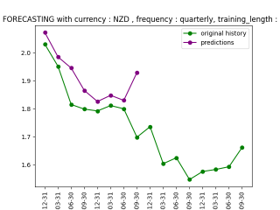
\includegraphics[width=\linewidth]{plots/r1.png}
    \end{column}
    \begin{column}{0.25\textwidth}
        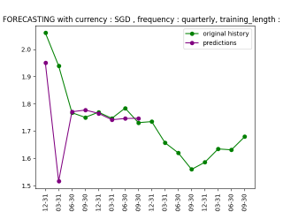
\includegraphics[width=\linewidth]{plots/r2.png}
    \end{column}
    \begin{column}{0.25\textwidth}
        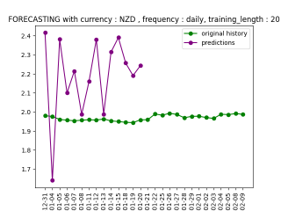
\includegraphics[width=\linewidth]{plots/r3.png}
    \end{column}
    \begin{column}{0.25\textwidth}
        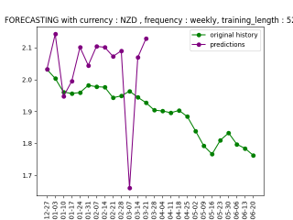
\includegraphics[width=\linewidth]{plots/r4.png}
    \end{column}
\end{columns}
\newpage

Model struggles with unpredictable currencies like \textit{USD} and \textit{GBP}.
\begin{columns}
    \begin{column}{0.5\textwidth}
        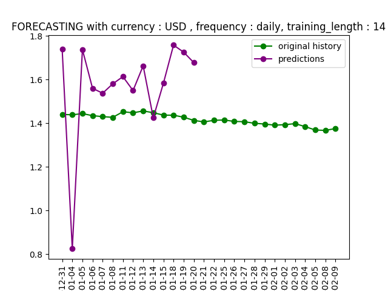
\includegraphics[width=\linewidth]{plots/usd-d.png}
    \end{column}
    \begin{column}{0.5\textwidth}
        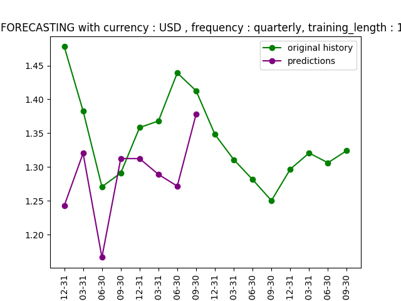
\includegraphics[width=\linewidth]{plots/usd-r.png}
    \end{column}
\end{columns}

\end{frame}

\section{Exponentially Smoothed Recurrent Neural Network}

\begin{frame}{ES-RNN: Origin and basic idea}
    
\end{frame}

\begin{frame}{ES-RNN: Holts-Winters model}
    
\end{frame}

\begin{frame}[fragile]{ES-RNN: Architecture}
    \begin{figure}[htbp]
    \centering
    \def\svgwidth{\columnwidth}
    \includesvg{./plots/es-rnn.svg}
    \end{figure}
\end{frame}

\begin{frame}[allowframebreaks]{ES-RNN: Training}
    
\end{frame}

\begin{frame}[allowframebreaks]{ES-RNN: Results}
    
\end{frame}

\begin{frame}[allowframebreaks]{References}

  \bibliography{demo}
  \bibliographystyle{abbrv}

\end{frame}

\end{document}
